\documentclass{my_paper}
\usepackage{ctex}
\usepackage[textwidth=444bp,vmargin=2.5cm]{geometry}%设置页边距
\usepackage{array} %主要是增加列样式选项
\usepackage[dvipsnames]{xcolor}%颜色宏包
\usepackage{graphicx}%图片宏包
\usepackage{amsmath}%公式宏包
\usepackage[T1]{fontenc}    
\usepackage{newtxtext, newtxmath}  %两种使用Times New Roman 字体的方法
\usepackage{subfigure}
\usepackage { gensymb }
% 打°符号\degree
\usepackage{listings}
% 代码
\usepackage{tabularx, booktabs} %% Load packages that you use
\usepackage{multirow} %跨行处理
\begin{document}

\newpage
\begin{center}
\lunwenbiaoti

\vspace{2ex}
\zhaiyao
\end{center}

摘要

\begin{guanjianci}
 元胞自动机 \quad 边缘检测 \quad 形状匹配
\end{guanjianci}

%----------- 正文 ----------
%----------- 一、问题重述 ----------
\newpage
\section{一、问题重述}

\subsection{问题背景}

一些背景

\subsection{问题重述}
经过分析整理,我们需要解决以下问题:
\begin{enumerate}
    \item 考虑到
    \item 在自卸
    \item 在第二
\end{enumerate}
\section{二、问题分析}
\subsection{问题一的分析}

该问要求我们查阅参考资料,建立战机机动的量化模型。为此考虑根据已知的飞行参数确定对应的战斗机机动行为。一个战斗行为可能来带一系列参数的变化,因此结合多个参数的变化情况来判断动作类型,对于某些复杂动作,可能会有多段变化过程,因此需要结合相邻的两次变化情况进行判断。由于决定飞机飞行动作的参数种类有限,每一种参数也只有集中情况,考虑就飞行参数变化建立决策树,对战斗机的机动行为进行识别。

\subsection{问题二的分析}

分析题中附件所给数据,得出附件中信息有以下特点:数据冗余、数据缺失和个体多样问题。针对数据冗余问题,需要去除那些不便于利用的数据格式;针对数据缺失问题,需要采用缺失处相邻部分的数据进行填充,考虑到填充过程不应当引入噪声,因此采用matlab工具箱中的移动均值方法填补缺失数据;对于数据个体多样问题,由于每个个体的动作分析应当独立进行,且需要分析的个体类型为“Air+FixedWing”且每次战斗不止有一架飞机参与战斗,因此需要使用id和类型对时间序列进行分类分析。

在分析数据的基础上,我们还构思了提取飞行参数变化情况的方法。单一飞机一段时间内的飞行数据,可以看作是多维度的时间序列数据。为了分析各个维度的变化状态,尝试使用差分法,但是体现出易受噪声干扰和局部性的特点,不能很好体现出数据的变化趋势。由于以上原因,又改用双滑动窗口法,具有较好的消除噪声和判断趋势的能力。

\subsection{问题三的分析}


%----------- 三、模型假设 ----------
\section{三、模型假设}
%使用代码片段:、jiashe%
\begin{enumerate}
    \item 飞机所记录的飞行参数真实可信,没有因各种因素而导致数据错误。
    
    \textbf{原因:}动作序列的分割识别工作基于飞行时的各项参数所决定,如果飞行参数有误,那么所计算得出的动作序列将不准确。

    \item 十大
    
    \textbf{原因:}
    
\end{enumerate}

%----------- 四、符号说明 ----------
\section{四、名词解释与符号说明}
%使用三线表格最好~
\subsection{名词解释}
\begin{enumerate}
    % 名词:、mingci
    \item \textbf{飞行参数}
    
    在空战模拟中飞机的时序数据,包含飞机海拔高度,真实空速(TAS),俯仰角,偏航角(Yaw)等指标。每条指标由id与Unix时间唯一标识。
    
    \item \textbf{机动动作}
    
    战机在空中飞行过程中,飞机为了某些战术意图而做出的行为。在分析过程中,机动动作是最小的分析单位,不能再进行分割。

    
\end{enumerate}
\subsection{符号说明}
以下是本文使用的符号以及含义:
\begin{table}[h]%htbp表示的意思是latex会尽量满足排在前面的浮动格式,就是h-t-b-p这个顺序,让排版的效果尽量好。
    \centering
    \begin{tabular}{p{2.0cm}<{\centering}p{9.0cm}<{\centering}p{2.0cm}<{\centering}}
 %指定单元格宽度, 并且水平居中。
    \hline
    符号 & 说明 & 单位 \\ %换行 
    \hline
    $L_0$ & 仓库长度 &  $m$\\
    
    \hline
    \end{tabular}
\end{table}

%----------- 五、模型的建立与求解 ----------
\section{五、模型的建立与求解}

以下将对提出的三个问题进行建模求解。

\subsection{机动动作描述与量化模型}

为了进行空战势态感知,机动决策,意图识别等工作,常常根据需要预先建立空战动作库\cite{1}。常见的空战库设计有两种方法,分别是包含丰富战术动作的典型战术动作库和由美国NASA学者\cite{2}提出的基本操纵动作库。前者内容丰富,但是前一种方法存在识别困难,对于某些复杂动作可能中断的情况处理不佳,而后一种方式以极限情况操作粗猛,不能保证组合出所有的战术动作。文献\cite{3}中提出的机动动作集合兼顾二者的优点,列举了仪表动作,简单特技,复杂特技共三类十二种动作,如表(\ref{dongzuo}) 。这一选择兼顾了简单动作与复杂动作,具有飞行动作代表性,易于识别。

\begin{table}[h]%htbp表示的意思是latex会尽量满足排在前面的浮动格式,就是h-t-b-p这个顺序,让排版的效果尽量好。
    \centering
    \caption{战斗机的三类机动动作}
    \vspace{10pt}
    \begin{tabular}{p{4.0cm}<{\centering}p{4.0cm}<{\centering}p{4.0cm}<{\centering}}
 %指定单元格宽度, 并且水平居中。
    \hline
    仪表动作 & 简单特技 & 复杂特技 \\ %换行 
    \hline
    盘旋 & \multirow{2}*{半滚倒转} & \multirow{2}*{“S”形急转} \\
    急跃升 &  &  \\
    俯冲 & \multirow{2}*{斤斗} & \multirow{2}*{战斗转弯} \\
     水平匀速直线飞行&  &  \\
     水平加速直线飞行& \multirow{2}*{半斤斗翻转} & \multirow{2}*{眼镜蛇机动} \\
     水平减速直线飞行&  &  \\

    \hline
    \end{tabular}
    \label{dongzuo}
\end{table}

\newpage 
下面分别介绍各个动作的战机移动特点,并总结出各个动作的定性判别标准。
\begin{enumerate}
    \item \textbf{盘旋}
    
    据有关文献\cite{4},盘旋动作时,飞机的航向角一定会发生变化。航向角变化是盘旋的主要特点,根据航向角的变化趋势,还可以将盘旋进一步细分为左盘旋和右盘旋。此外,盘旋还可以被分为各种细类,但是考虑到识别的效率和复杂度,本文中仅考虑水平稳定盘旋,在此过程中,飞机飞行速度和飞行高度俱不变。

    \item \textbf{急跃升}
    
    在急跃升动作中,飞机迅速拉起,以达到躲避敌机和占据有利地位的目的。其飞行参数特点是提升高度的同时降低了速度。
    \item \textbf{俯冲}
    
    飞机进行俯冲动作时以大角度和高速度下冲,在飞机高度下降过程中飞机的势能转变为机械能,速度增加。
    \item \textbf{直线飞行}
    
    飞行过程中高度和方位角不发生变化,此时飞机进行直线飞行。根据加速度分为加速、匀速和减速直线飞行三种。

    \item \textbf{半滚倒转}
    
    据参考文献显示\cite{5},半滚倒转是一种常用在脱离空战情况下的机动方式。在进行该动作时,飞机先横滚半圈,再做半个内斤斗,随后在低高度下反方向改平飞出,如图(\ref{dz}a) 。该机动方式迅速改变航向的同时,降低了高度,提升速度,是一种高效的脱离方式。

    \item \textbf{斤斗}
    
    在斤斗过程中,飞机由水平直线飞行过程中拉起机身,在竖直方向上做一个圆周运动,飞机机盖指向圆周内部,如图(\ref{dz}b)。飞行参数表现为高度先升高后降低,航向角发生两次突变,速度先增后减。

    \begin{figure}[htbp]
        \centering  %居中
        \subfigure[半滚倒转示意图]{   %第一张子图
        \begin{minipage}{0.4\textwidth}%大小总和超过textwidth则自动换行
        \centering    %子图居中
        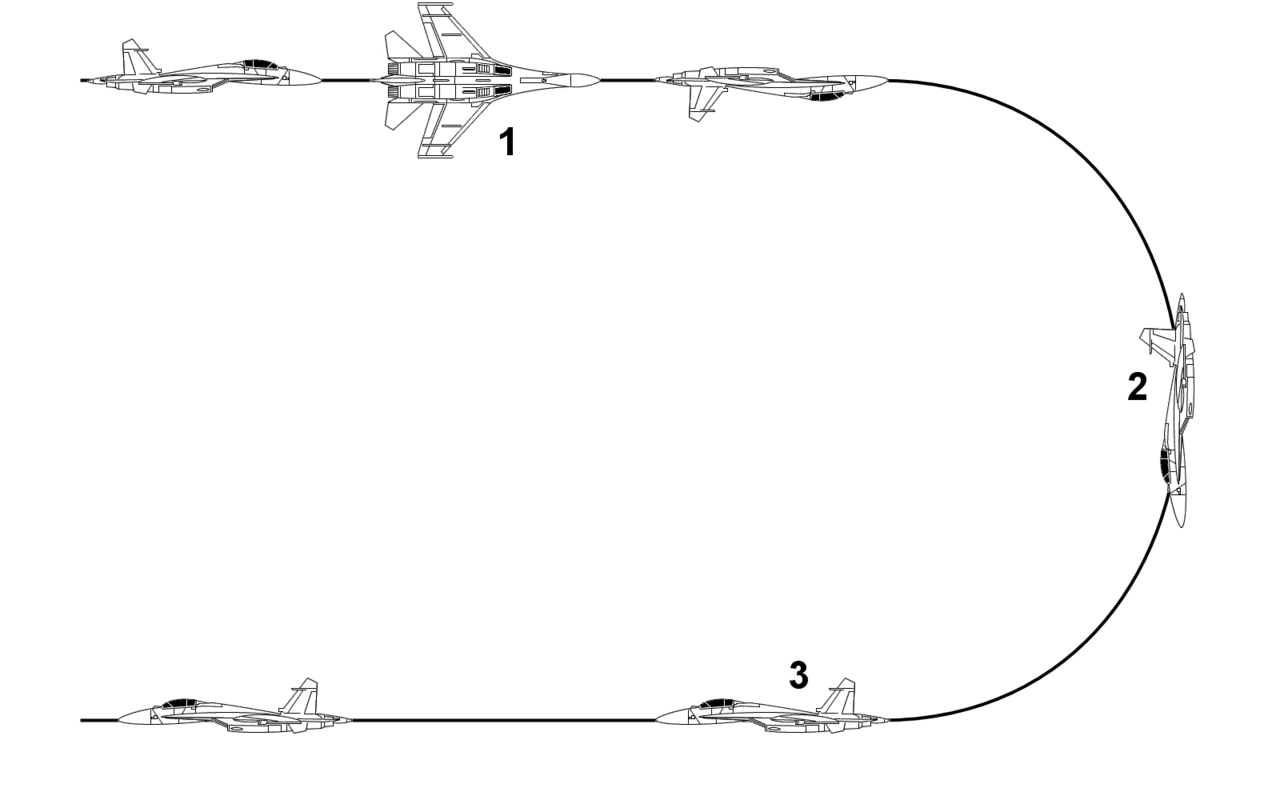
\includegraphics[width=\textwidth]{bangun.png}  %设置图片的输出大小倍数,这里是0.5倍大小输出
        \end{minipage}
        }
        \subfigure[斤斗示意图]{ %第二张子图
        \begin{minipage}{0.4\textwidth}
        \centering    %子图居中
        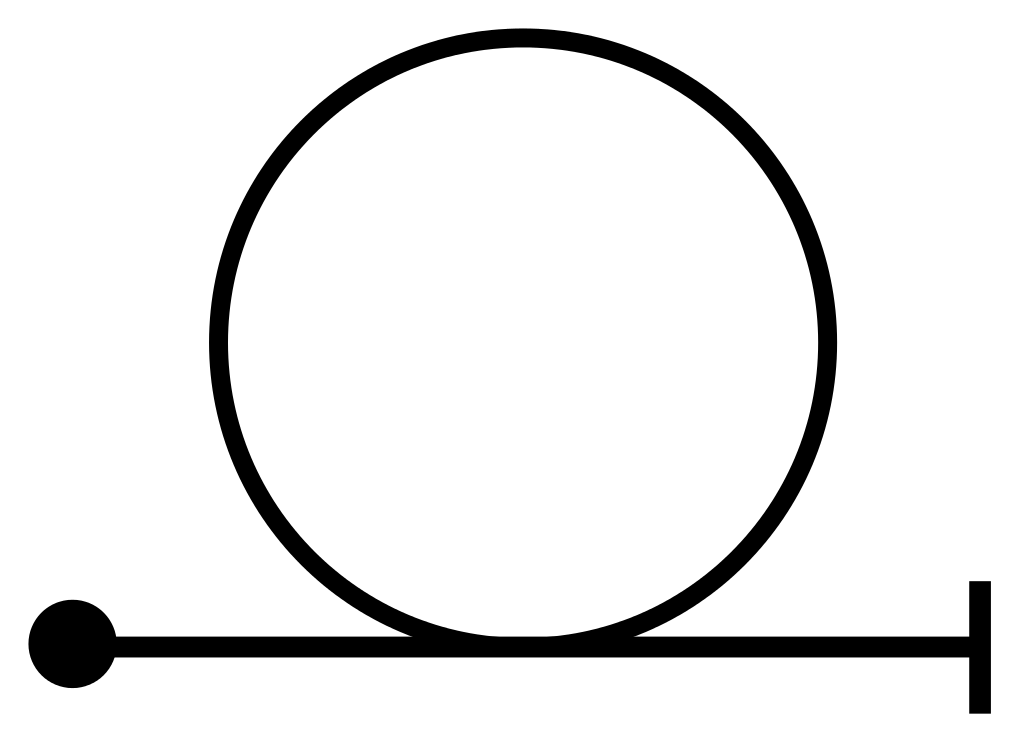
\includegraphics[width=\textwidth]{jindou.png}%以pic.jpg的0.5倍大小输出
        \end{minipage}
        }
            \subfigure[眼镜蛇机动示意图]{   %子图
            \begin{minipage}{0.4\textwidth}%大小总和超过textwidth则自动换行
            \centering    %子图居中
            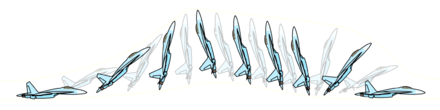
\includegraphics[width=\textwidth]{yjs.png}  %设置图片的输出大小倍数,这里是0.5倍大小输出
            \end{minipage}
            }        
    
        \caption{部分飞行动作示意图}    %大图名称
        \label{dz}    %图片引用标记
    \end{figure}
    
    \item \textbf{“S”形急转}
    
    飞机在进行“S”形急转时方向变化两次,高度不发生变化。经过该动作后的飞机航向改变。

    \item \textbf{战术转弯}
    
    该动作适用于在俯冲攻击后改出的情况,在拉升的过程中同时改变方向角。在此过程中,高度上升,方向角增加或者减少。

    \item \textbf{眼镜蛇机动}
    
    在敌机紧追我方时使用该动作对敌方进行战术躲避。\cite{7}该动作上拉机头,导致飞行速度迅速降低,随后机头开始下沉时,加大油门直到飞机转为水平姿态。在整个过程中,飞机的高度基本保持不变,如图(\ref{dz}c)所示 。
    
\end{enumerate}

为了区分各个机动动作,综合上述分析结果,文章还提出各动作的定性评价指标。所列出的十二项动作都可以由五项飞行参数定量确定,这些参数同附件二中的信息对应情况如下表所示:
\section{七、模型的评价}

\subsection{模型的优点}
\begin{enumerate}
    \item 采用

\end{enumerate}

\subsection{模型的缺点}
\begin{itemize}
    \item 利用较

\end{itemize}

%----------- 参考文献 ----------
\newpage
\bibliographystyle{unsrt} %规定了参考文献的格式
\begin{center}
\bibliography{reference} %调出LaTeX生成参考文献列表
\end{center}

%----------- 附录 ----------
\newpage
\section{附件}
\textbf{附件清单:}
\begin{itemize}
    \item xxx代码
\end{itemize}

\textbf{sobel边缘检测代码}

\begin{lstlisting}[language=matlab]
    function GAdsa 
\end{lstlisting}



\end{document}